\documentclass[aspectratio=169]{beamer}
% Shared Beamer style for this repository.
\usepackage[fontset=none]{ctex}
\usepackage{fontspec}
\setmainfont{DejaVu Serif}
\setsansfont{DejaVu Sans}
\setmonofont{DejaVu Sans Mono}
\setCJKmainfont{Noto Serif CJK SC}[BoldFont={Noto Serif CJK SC Bold}]
\setCJKsansfont{Noto Sans CJK SC}[BoldFont={Noto Sans CJK SC Bold}]
\setCJKmonofont{Noto Sans Mono CJK SC}

\usetheme{Madrid}
\usefonttheme{serif}
\setbeamertemplate{navigation symbols}{}
\setbeamertemplate{footline}[frame number]

\usepackage{graphicx}
\usepackage{amsmath,amssymb}
\usepackage{booktabs}
\usepackage{array}
\usepackage{xcolor}
\usepackage{listings}
\usepackage{tikz}
\usetikzlibrary{shapes,arrows,positioning}

% Color system
\definecolor{dcPrimary}{RGB}{21,101,117}
\definecolor{dcSecondary}{RGB}{140,115,72}
\definecolor{dcAccent}{RGB}{184,92,63}
\definecolor{dcMuted}{RGB}{230,250,252}
\definecolor{dcWarmBG}{RGB}{255,245,230}
\definecolor{dcCodeBG}{RGB}{247,248,250}
\definecolor{dcCodeFrame}{RGB}{200,210,215}

\setbeamercolor{structure}{fg=dcPrimary}
\setbeamercolor{palette primary}{fg=dcPrimary,bg=dcMuted}
\setbeamercolor{palette secondary}{fg=dcSecondary,bg=dcMuted!90}
\setbeamercolor{palette tertiary}{fg=dcPrimary,bg=dcMuted!80}
\setbeamercolor{frametitle}{fg=white,bg=dcPrimary}
\setbeamercolor{title}{fg=dcPrimary}
\setbeamercolor{alerted text}{fg=dcAccent}
\setbeamercolor{item}{fg=dcPrimary}
\setbeamercolor{subitem}{fg=dcSecondary}
\setbeamercolor{block title}{fg=white,bg=dcPrimary}
\setbeamercolor{block body}{bg=dcMuted}
\setbeamercolor{block title example}{fg=white,bg=dcSecondary}
\setbeamercolor{block body example}{bg=dcWarmBG}
\setbeamercolor{block title alerted}{fg=white,bg=dcAccent}
\setbeamercolor{block body alerted}{bg=dcWarmBG}
\setbeamercolor{footline}{fg=dcPrimary}

\lstset{
  basicstyle=\ttfamily\footnotesize,
  backgroundcolor=\color{dcCodeBG},
  frame=single,
  rulecolor=\color{dcCodeFrame},
  numbers=none,
  breaklines=true,
  showstringspaces=false,
  tabsize=2
}


\title{时序逻辑、状态机与时序约束基础}
\subtitle{第三章第二讲：从寄存器边界、状态机到 setup/hold 与亚稳态}
\author{Digital Circuit Getting Started}
\date{\today}

\graphicspath{{figures/}}

\begin{document}

\begin{frame}
  \titlepage
\end{frame}

\begin{frame}{Learning Objectives}
\begin{itemize}
  \item 理解组合逻辑与时序逻辑的语义差异：前者是映射，后者是状态演化
  \item 区分 latch、flip-flop、register、register chain 与 state machine 的作用
  \item 建立“寄存器边界 + 组合逻辑锥”的观察框架
  \item 理解 propagation delay、setup、hold、skew、uncertainty 与 metastability 的工程含义
\end{itemize}
\end{frame}

\begin{frame}{The Game Plan}
\begin{enumerate}
  \item 为什么引入寄存器后，系统语义就变了
  \item latch / flop / register 分别在解决什么问题
  \item 状态机怎样把状态寄存器、下一状态逻辑和输出逻辑接起来
  \item setup / hold / skew / uncertainty 为什么是同步系统的成立条件
  \item 异步输入与跨时钟域为什么会挑战数字抽象
\end{enumerate}
\end{frame}

\begin{frame}{Combinational vs. Sequential Semantics}
\begin{columns}[T]
  \column{0.48\linewidth}
  \begin{block}{组合逻辑}
  \small
  当前输出只依赖当前输入。\newline
  语义更像一个函数：\texttt{y = f(x)}。
  \end{block}

  \column{0.48\linewidth}
  \begin{block}{时序逻辑}
  \small
  当前输出还依赖过去保存下来的状态。\newline
  语义更像状态转移：\texttt{state[n+1] = g(state[n], in[n])}。
  \end{block}
\end{columns}

\vspace{0.7em}
\textbf{一旦引入寄存器，系统就不再只是“当前输入到当前输出”的映射。}
\end{frame}

\begin{frame}{Latch, Flip-Flop, Register}
\begin{columns}[T]
  \column{0.52\linewidth}
  \centering
  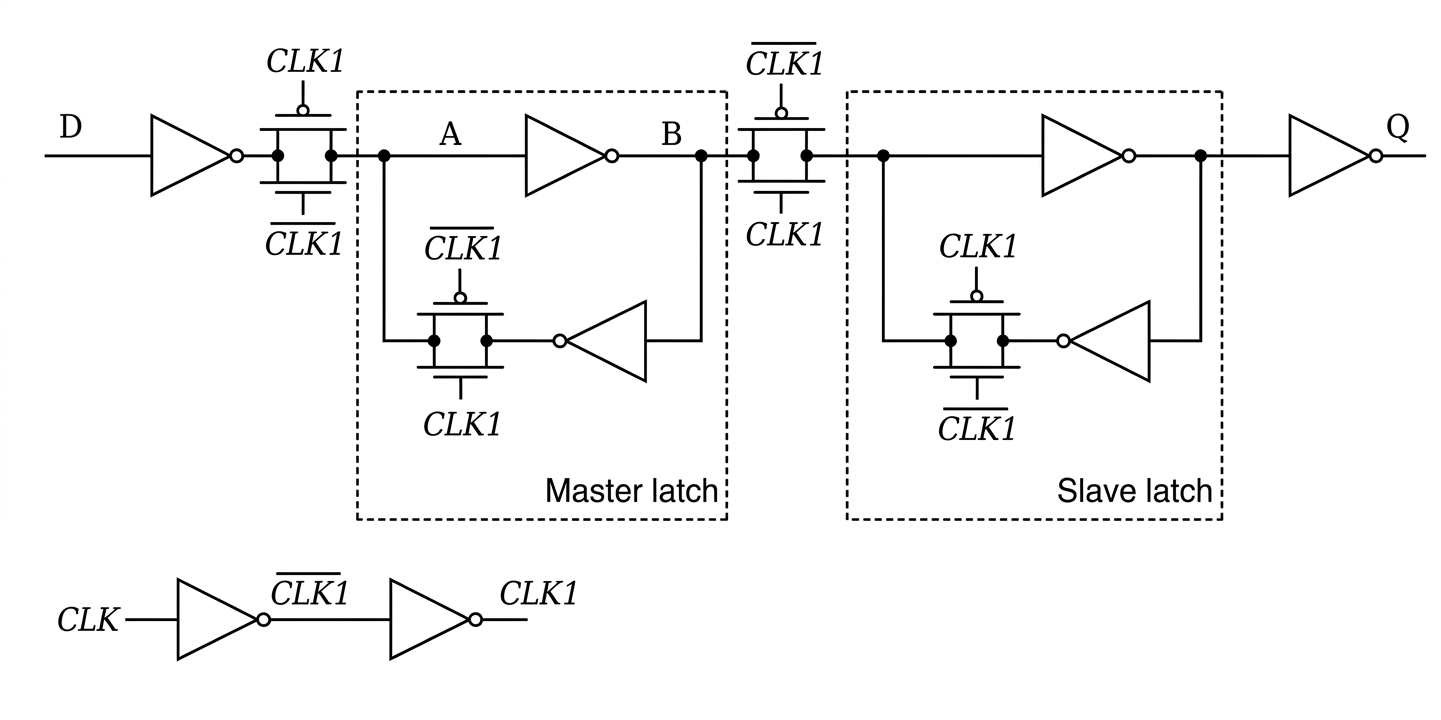
\includegraphics[width=0.92\linewidth]{flipflop_ms.png}
  \column{0.44\linewidth}
  \small
  \begin{itemize}
    \item \textbf{Latch}：电平敏感，门控期间输入变化可能继续传到输出
    \item \textbf{Flip-flop}：边沿敏感，在时钟边沿附近采样
    \item \textbf{Register}：一组并行触发器，用来保存多位状态
    \item \textbf{Register chain}：多个寄存器首尾相接，用来切分路径或同步数据
  \end{itemize}
\end{columns}
\end{frame}

\begin{frame}{The Register-Logic-Register View}
\begin{columns}[T]
  \column{0.52\linewidth}
  \centering
  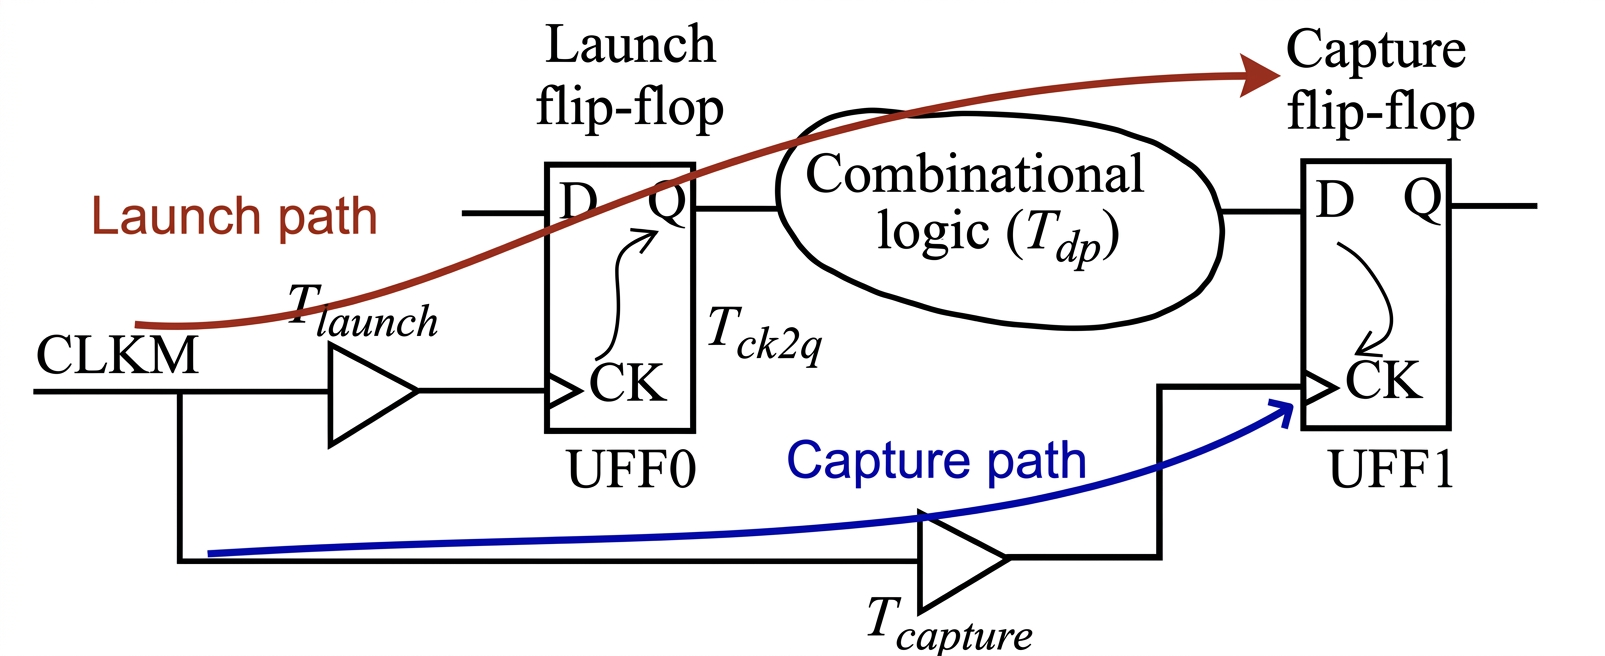
\includegraphics[width=0.94\linewidth]{reg_logic_reg.png}
  \column{0.44\linewidth}
  \small
  \begin{itemize}
    \item 同步系统最常见的观察框架：寄存器 $\rightarrow$ 组合逻辑锥 $\rightarrow$ 寄存器
    \item 左边寄存器负责发射数据，右边寄存器负责捕获数据
    \item 中间组合逻辑必须在允许的时间窗口内收敛
    \item 时序分析本质上是在检查这些边界是否可靠
  \end{itemize}
\end{columns}
\end{frame}

\begin{frame}{State Machine Anatomy}
\begin{columns}[T]
  \column{0.50\linewidth}
  \centering
  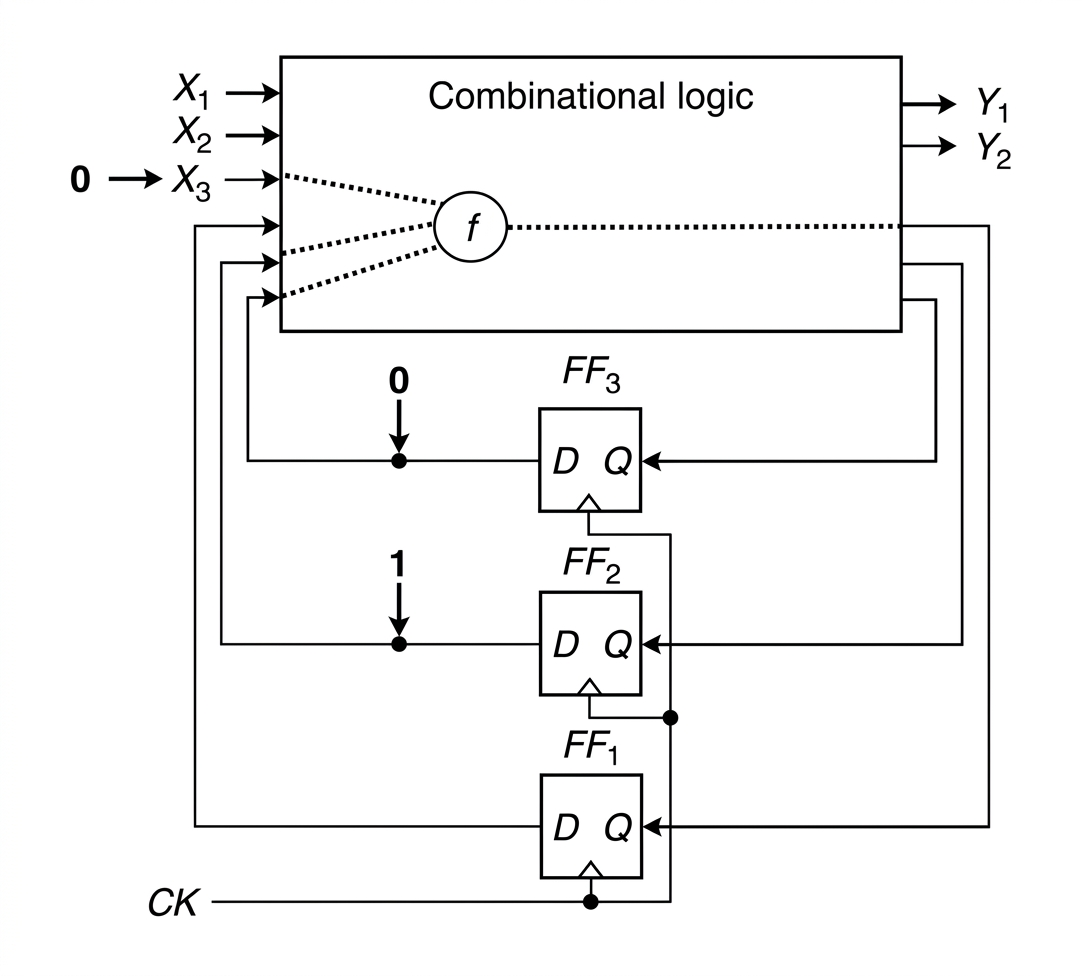
\includegraphics[width=0.92\linewidth]{mealy.jpeg}
  \column{0.46\linewidth}
  \small
  \begin{itemize}
    \item 状态机通常由三部分组成：状态寄存器、下一状态逻辑、输出逻辑
    \item Moore 机：输出主要由状态决定
    \item Mealy 机：输出可同时受当前状态与输入影响
    \item Moore / Mealy 差异不是背定义，而是观察输出何时变化、是否更容易受输入毛刺影响
  \end{itemize}
\end{columns}
\end{frame}

\begin{frame}{Propagation Delay, Setup, Hold}
\begin{columns}[T]
  \column{0.52\linewidth}
  \centering
  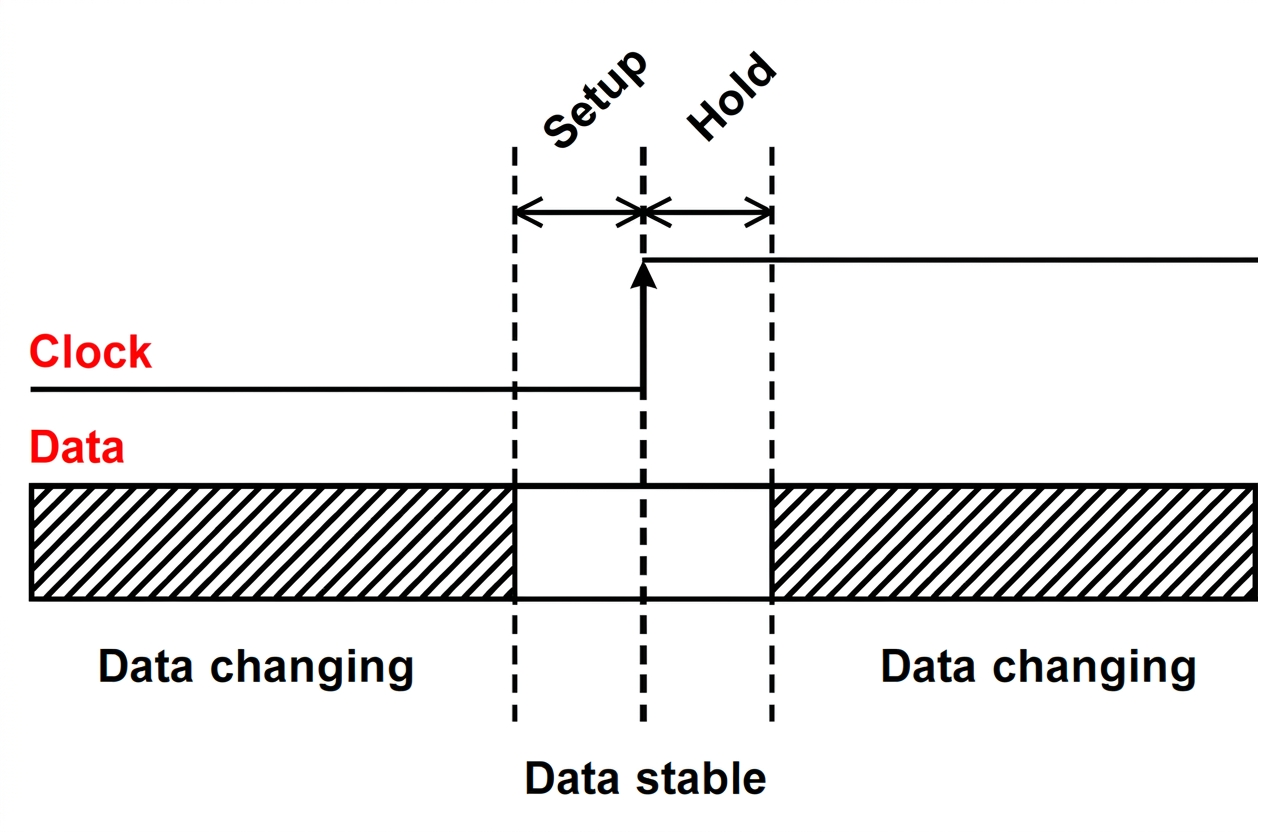
\includegraphics[width=0.94\linewidth]{setup_hold.png}
  \column{0.44\linewidth}
  \small
  \begin{itemize}
    \item \textbf{Propagation delay}：数据从起点寄存器穿过逻辑到达终点的时间
    \item \textbf{Setup time}：采样边沿到来前，数据必须提前稳定一段时间
    \item \textbf{Hold time}：采样边沿过后，数据还必须继续保持一段时间
    \item 这两个窗口不是礼貌性建议，而是触发器可靠采样的边界条件
  \end{itemize}
\end{columns}
\end{frame}

\begin{frame}{What a Setup Violation Means}
\small
\begin{itemize}
  \item 数据路径太慢、时钟周期太短、skew 太不利，都可能让数据在采样前还没稳定
  \item 结果不是“略微不准一点”，而是终点寄存器可能采到旧值、错值，甚至进入亚稳态
  \item 所以提高频率并不只是把数字写大，而是在压缩每条组合路径的收敛时间
\end{itemize}

\vspace{0.6em}
\textbf{一句话：setup 违例说明这个周期内该完成的计算，还没来得及完成。}
\end{frame}

\begin{frame}{What a Hold Violation Means}
\small
\begin{itemize}
  \item 数据路径太快、时钟到达差异过大，可能让新数据在采样后立刻冲到终点寄存器
  \item 终点寄存器还没关上采样窗口，就被下一份数据污染
  \item hold 问题往往和“最短路径”有关，修法也常与 setup 问题不同
\end{itemize}

\vspace{0.6em}
\textbf{一句话：hold 违例说明上一拍刚被采走的数据，还没来得及稳住就被下一拍推翻。}
\end{frame}

\begin{frame}{Skew and Uncertainty}
\begin{columns}[T]
  \column{0.48\linewidth}
  \begin{itemize}
    \item \textbf{Clock skew}：同一时钟边沿并不是同时到达所有寄存器
    \item 正 skew、负 skew 会分别影响 setup / hold 裕量
    \item \textbf{Clock uncertainty}：抖动、建模误差、分布变化等带来的额外不确定性
  \end{itemize}
  \column{0.48\linewidth}
  \begin{alertblock}{关键结论}
  \small
  时钟不是一根“全芯片同时生效”的理想魔法线。\newline
  时钟本身也是一张需要被设计、约束和分析的物理网络。
  \end{alertblock}
\end{columns}
\end{frame}

\begin{frame}{Timing Is Still Coupled to Load and Transition}
\small
\begin{itemize}
  \item 前一讲提到的 fanout、负载、transition、rise/fall time，在这里继续影响整条寄存器到寄存器路径
  \item 组合逻辑锥越深、负载越重、边沿越慢，setup 压力通常越大
  \item 时序约束并不是脱离电路结构单独存在的公式，它们是在总结真实实现的行为边界
\end{itemize}
\end{frame}

\begin{frame}{Metastability: The Forbidden Middle Can Be Touched}
\begin{columns}[T]
  \column{0.48\linewidth}
  \centering
  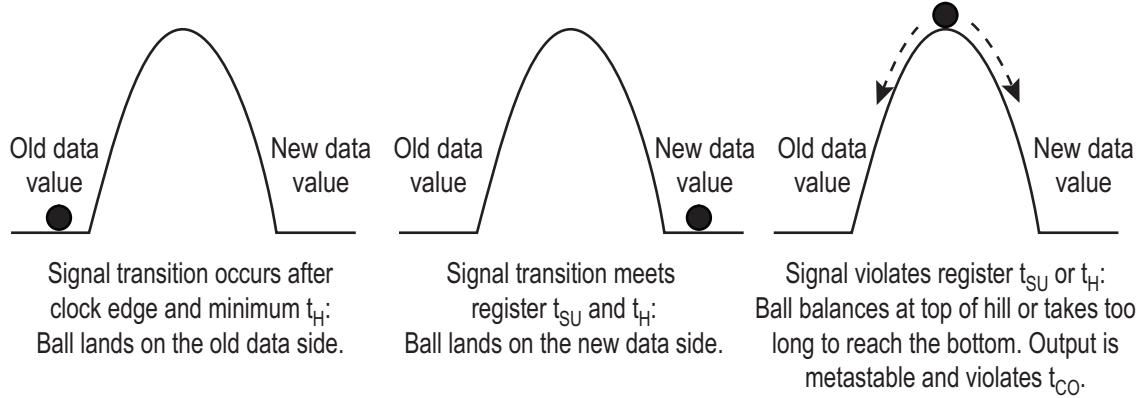
\includegraphics[width=0.92\linewidth]{metastability_description.jpg}
  \column{0.48\linewidth}
  \small
  \begin{itemize}
    \item 如果输入在采样窗口附近变化，触发器内部可能短时间无法决定输出该去 0 还是 1
    \item 这不是第三种稳定逻辑值，而是一种不稳定的过渡状态
    \item 它最终通常会收敛，但收敛时间不可被完全上界化
  \end{itemize}

  \vspace{0.4em}
  \textbf{亚稳态不能被“消灭”，只能通过设计把概率压低。}
\end{columns}
\end{frame}

\begin{frame}{Metastability Is a Probability Problem}
\begin{columns}[T]
  \column{0.50\linewidth}
  \centering
  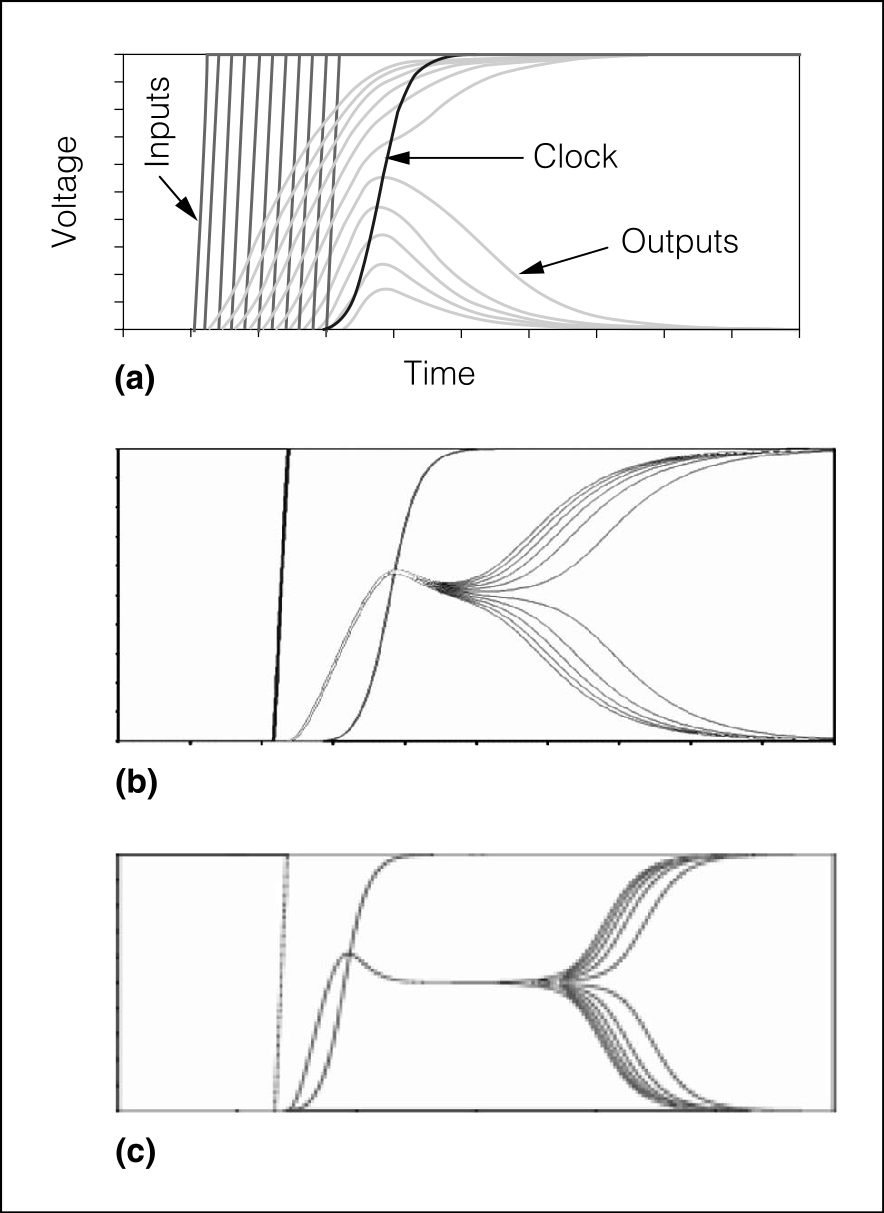
\includegraphics[width=0.92\linewidth]{metastability_sim.png}
  \column{0.46\linewidth}
  \small
  \begin{itemize}
    \item 异步输入永远可能在“坏时刻”撞上采样边沿
    \item 工程目标不是承诺零概率，而是把平均失效间隔拉到系统可接受范围外
    \item 因此 CDC 设计、同步器级数、时钟频率和输入事件率都会进入风险预算
  \end{itemize}
\end{columns}
\end{frame}

\begin{frame}{Clock Domain Crossing and the 2-FF Synchronizer}
\begin{columns}[T]
  \column{0.50\linewidth}
  \centering
  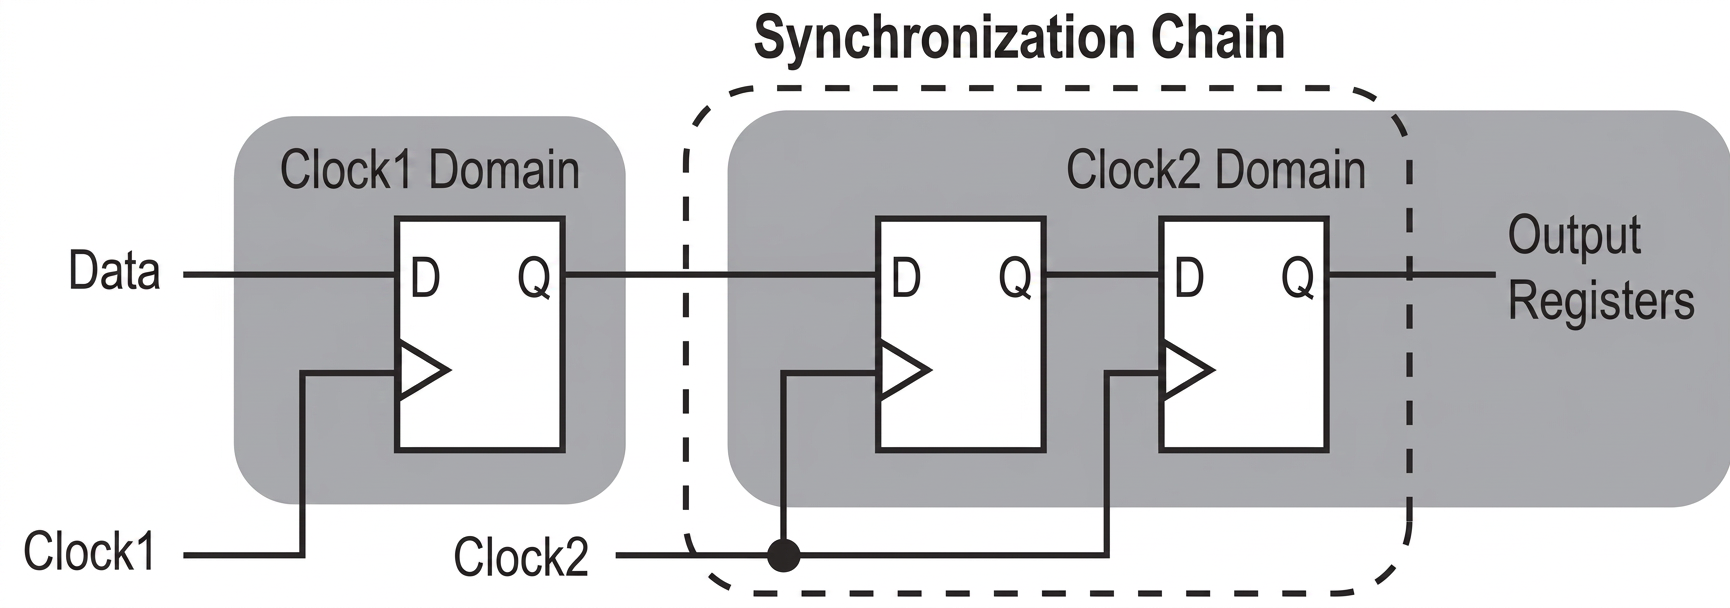
\includegraphics[width=0.88\linewidth]{dual_dff_capture.png}
  \column{0.46\linewidth}
  \small
  \begin{itemize}
    \item 双触发器同步器的作用：给可能亚稳的第一级触发器多一拍恢复时间
    \item 它适合单 bit 控制信号，不适合直接搬运多 bit 总线语义
    \item 它降低风险，但不保证逻辑协议自动正确
  \end{itemize}

  \vspace{0.4em}
  \textbf{同步器解决的是概率问题，不是协议问题。}
\end{columns}
\end{frame}

\begin{frame}{Boundary Conditions to Remember}
\begin{itemize}
  \item “仿真没报错”不等于时序满足
  \item “逻辑表达式正确”不等于同步系统可靠
  \item “加了同步器”不等于所有跨域问题都解决
  \item 真正需要管理的是：状态边界、时间边界和同步边界
\end{itemize}
\end{frame}

\begin{frame}{Takeaways}
\begin{itemize}
  \item 寄存器把系统从组合语义推进到状态语义，状态机是这种组织方式的标准骨架
  \item setup / hold / skew / uncertainty 定义了同步系统能否可靠工作的时间边界
  \item metastability 提醒我们：异步世界总会挑战数字抽象，只能通过同步策略降低风险
  \item 进入下一章 RTL 之前，最重要的是先把这些语义边界看清楚，而不是急着背语法
\end{itemize}
\end{frame}

\begin{frame}{After-Class Prompt}
请完成三件事：
\begin{enumerate}
  \item 画出一个寄存器-组合逻辑-寄存器结构，并标出 setup / hold 检查窗口
  \item 给出一个简单状态机，说明哪些部分属于状态寄存器，哪些属于组合逻辑
  \item 解释为什么异步按键直接送入主时钟域寄存器会带来风险，双触发器同步器能解决什么、不能解决什么
\end{enumerate}
\end{frame}

\end{document}
